\documentclass[a4paper,10pt,twocolumn,uplatex]{jsarticle}
\usepackage{style/nislab,style/resume}

%---------------------------------------------------------------------
% レジュメ種別・日付設定(要変更)
% \type{} 1:修士論文諮問会 2:卒業論文発表会 3:月例発表会 4:研究室合同発表会
%---------------------------------------------------------------------
\type{3}
\year{2022}
\month{10}
\date{8}

%---------------------------------------------------------------------
% ページ番号設定(要変更)
%---------------------------------------------------------------------
\setcounter{page}{1}

%---------------------------------------------------------------------
% 変更不要
%---------------------------------------------------------------------
\begin{document}

%---------------------------------------------------------------------
% タイトル作成部分(要変更)
% \maketitle{タイトル}{title}{名前}{name}
%---------------------------------------------------------------------
\maketitle{SDNを利用したQoS予測・予約によるV2X通信の信頼性向上}
{Improvement of V2X Communication Reliability\\by QoS Prediction \& Reservation Using SDN}
{国本 典晟}
{Tensei KUNIMOTO}

%---------------------------------------------------------------------
\section{はじめに}
協調型自動運転の実現に向けて,車両とあらゆるものを接続するV2X(Vehicle to Everything)通信の研究が積極的に行われている.
安全かつ効率的な走行のため,車両は基地局を介してインターネット上のクラウドサーバや基地局近くなどに地理的に分散配置されたエッジサーバと通信を行い,必要な情報を得る.
しかし,今後交通サービスを提供するアプリケーションの増加や自動運転車両の普及が進む中で,ある基地局を介してエッジサーバと通信する車両が,そこで利用可能な通信帯域で収容可能な車両台数以上に集中した場合に,通信のQoS(Quality of Service)を保証することができない事態が発生することが懸念されている.(参考文献)
事前にQoSが保証されないことを予測できなかった場合,協調型自動運転に必要な情報を受け取ることができないため,安全性の低下や旅行時間の増加といった問題が発生する.
また,他の車両よりも優先的に情報を受け取る必要がある緊急車両などのQoSを保証できない問題も想定される.\par
本研究では,ソフトウェアを介してネットワークを一元管理するSDN(Software Defined Networking)を利用することで,車両の移動を想定することでQoSを予測することを提案する.
QoSが保証できない場合には,QoS予測に基づき基地局のネットワークを制御する.
また,特定車両に対してQoSの予約を行うことを提案する.

%---------------------------------------------------------------------
\section{提案手法}
\subsection{SDNを利用したQoS予測}
\label{QoSprediction}
SDNを利用して車両の移動を想定する.
車両は現在地,速度,走行方向,移動計画を常にSDNコントローラへ送信する.
SDNコントローラは自身が管理する範囲内の地図情報と範囲内の基地局の位置と利用可能な通信帯域の情報を持つ.
SDNコントローラは車両の情報と地図情報を照らし合わせて車両の集中状況を予測する.
予測した集中状況と基地局の情報に基づき,基地局の利用可能な通信帯域で収容可能な台数以上の車両が集中していないかを判定することで,QoSを予測する.

\begin{figure}[t]
	\begin{centering}
    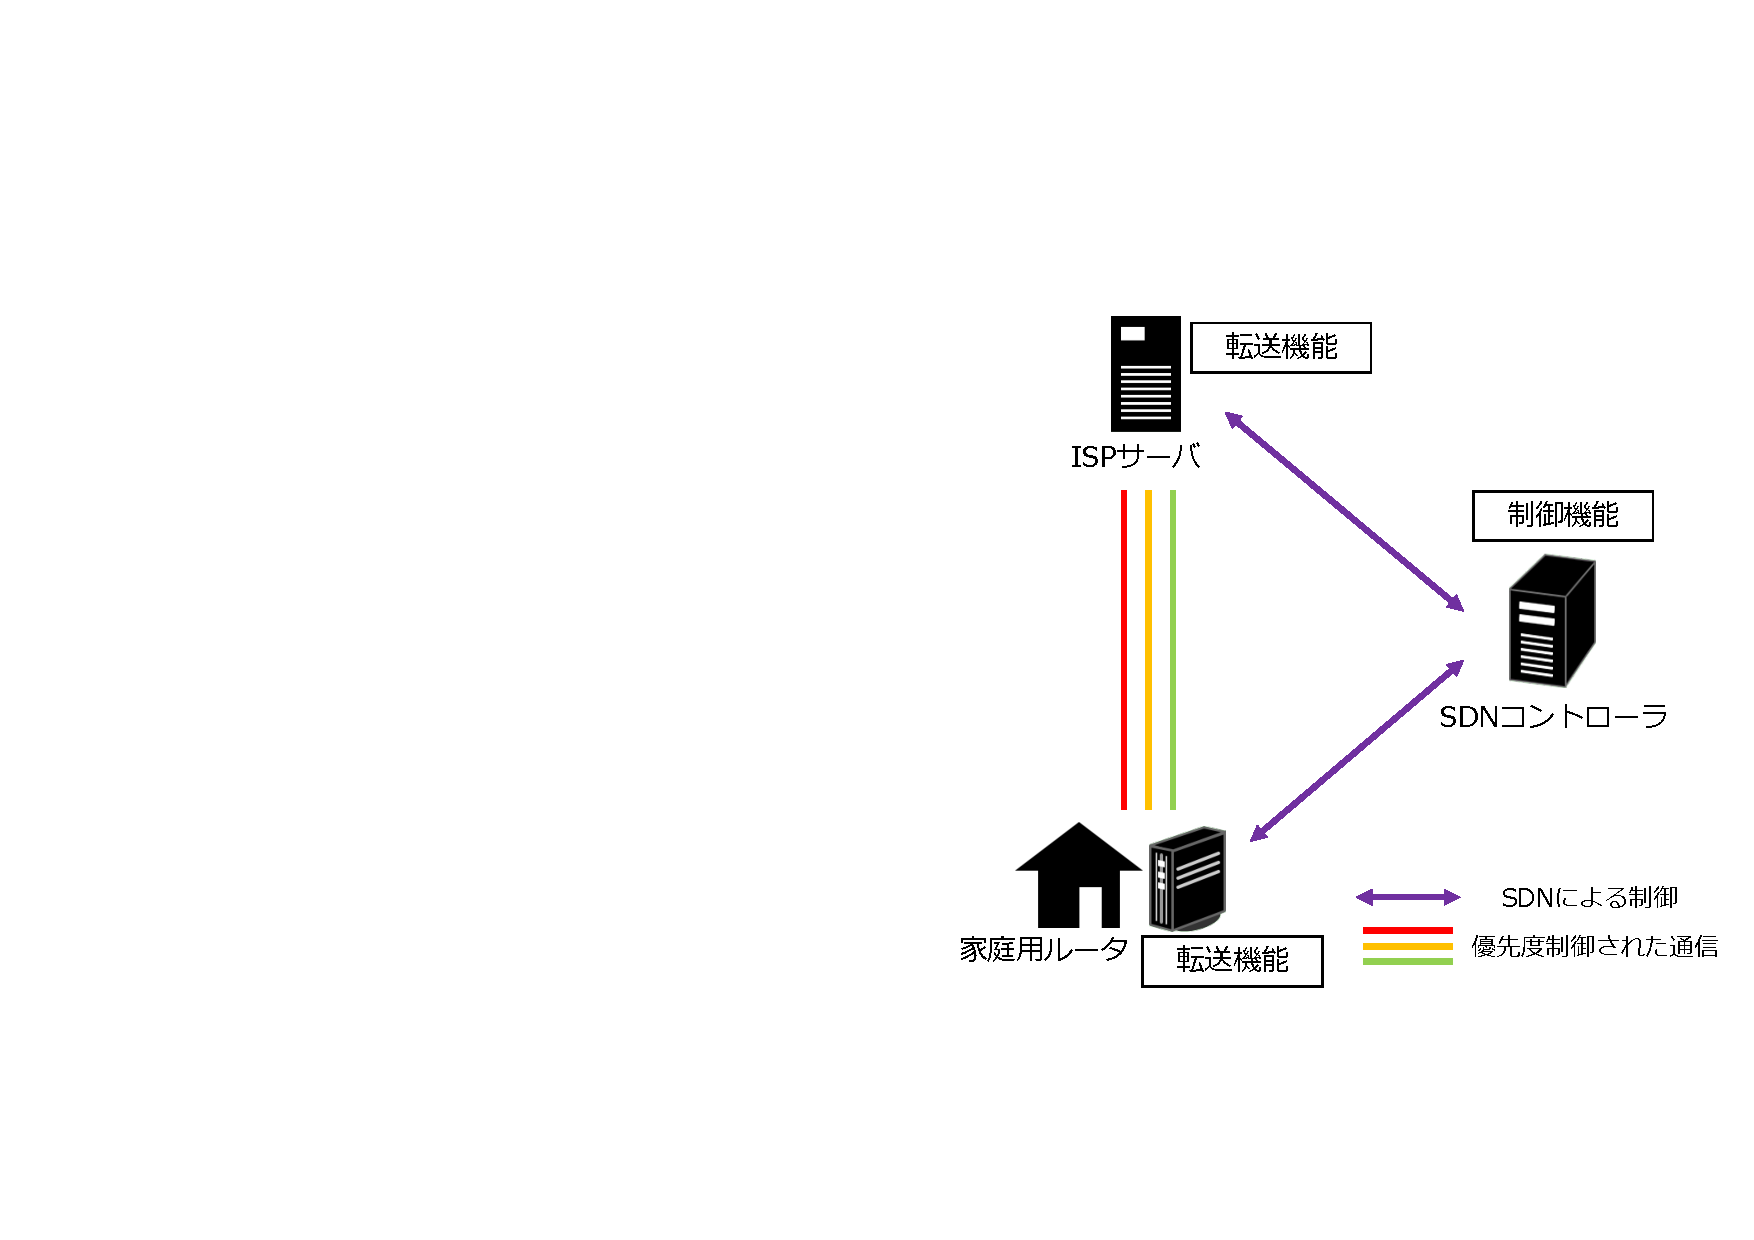
\includegraphics[width=0.7\linewidth]{img/proposal_resume.pdf}
    \caption{SDNを用いた通信制御}
    \label{fig:proposal}
    \end{centering}
\end{figure}

%---------------------------------------------------------------------
\subsection{QoS予測に基づくネットワーク制御}
\label{priority}
\ref{QoSprediction}節のQoS予測の結果,QoSの保証ができない場合,協調型自動運転に必要な情報を受け取ることができないため,自車両に搭載されたセンサのみを用いて慎重に走行する必要があり,旅行時間の増大が懸念される.
そこで,SDNコントローラはネットワーク制御を行うことでQoSの保証を目指す.
ある基地局において,利用可能な通信帯域で収容可能な台数以上に車両が集中している場合,収容可能な台数から超過している台数分の車両を,まだ利用可能な通信帯域に空きのある基地局の周辺を走行するよう経路を変更させることで,QoSを保証することができる.
しかし,経路を変更したために旅行時間が大きく増大し,変更前の経路を自車両のセンサのみを用いて慎重に走行した方が結果として旅行時間が短かった,という可能性がある.
そのため,経路ごとに旅行時間と通信する基地局の空き帯域をパラメータとしてコストを計算し,そのコストをもとに各車両の経路を決定する.\par

まず,SDNコントローラは

車両の走行経路
基地局(AP)とのやり取りも必要

%---------------------------------------------------------------------
\subsection{QoS予約}
緊急車両などの特定車両は,より安全で効率的な運転のため,他の車両よりも優先して情報を受け取る必要があるため,QoSを事前に保証しなければならない場合が想定される.
そこで,特定車両に対してQoSの予約を行うことを提案する.
QoS予約の手順を図に示す.

%---------------------------------------------------------------------
\subsection{提案手法の通信手順}
提案手法の通信手順を図に示す.
本当に分ける意味ある?

%---------------------------------------------------------------------
\section{シミュレーションによる評価}
\subsection{シミュレーションモデル}
提案手法の有効性を検証するため,図のような移動経路網モデルでシミュレーションを行う.
シミュレーションの条件は次の通りである.

シミュレーションモデルを図付きで説明
シミュレーションモデルの条件を説明

%---------------------------------------------------------------------
\subsection{評価項目}
時刻ごとの基地局周囲の車両台数を,提案手法を用いない場合と用いた場合を比較することにより,QoS保証について評価する.
基地局の利用可能な通信帯域で収容可能な台数以上の車両が基地局周囲のいる場合,QoSを保証できていないと考える.
また,経路ごとの旅行時間と通信する基地局の空き帯域をパラメータとしてコストを計算し経路を決定する手法について,提案手法を用いない場合と全車両の合計旅行時間を比較することにより評価を行う.

上と分ける必要ある?

%---------------------------------------------------------------------
\section{まとめと今後の課題}
V2X通信において,基地局周辺に車両が集中した場合,基地局の利用可能な通信帯域で収容可能な台数を超過し,QoSを保証できない問題が懸念されている.
本研究では,SDNを用いて車両の集中状況を予測することでQoSを予測し,QoS予測に基づき基地局のネットワークを制御することと,特定車両のQoSを予約することを提案した.
本研究ではコストを用いた経路の決定方法について評価するために簡易的なモデルにおいて評価を行うが,より安全で効率的な走行を行うために,基地局と通信できない車両に対して,車車間通信によって情報提供を行うことも併せて検討する必要があると考えている.

%---------------------------------------------------------------------
% Bibliography(参考文献)
%---------------------------------------------------------------------
% thebibliography を利用する場合は以下を使用
\footnotesize{
  \begin{thebibliography}{99}
    \bibitem{ガイドライン} 総務省,帯域制御の運用基準に関するガイドライン(改定), 2019.
    \bibitem{AQRA} Guo-Cin Deng and Kuochen Wang, An Application-aware QoS Routing Algorithm for SDN-based IoT Networking, \textit{2018 IEEE Symposium on Computers and Communications (ISCC)}, pp. 186-191, 2018.
  \end{thebibliography}
}

% BibTex を利用する場合は以下を使用(初めての人には難しいかも)
% \bibliographystyle{junsrt}
% \bibliography{myref}

%---------------------------------------------------------------------
\end{document}
%---------------------------------------------------------------------
